\section{Model Evaluation and Comparison}
\label{sec:model-evaluation}
\begingroup
\setlength{\emergencystretch}{3em}

\subsection{Evaluation Protocol}

The 359,551 test listings follow training observations from June--December 2025 and validation observations from December 2025--January 2026. Testing spans January--March 2026. Test targets are excluded from hyperparameter fitting, stopping decisions, and blend estimation.

For $n$ test observations, the four reported metrics are
\begin{align}
\operatorname{MAE} &= \frac{1}{n}\sum_{i=1}^{n}|y_i-\widehat{y}_i|,
&\operatorname{RMSE} &= \sqrt{\frac{1}{n}\sum_{i=1}^{n}(y_i-\widehat{y}_i)^2},\\
R^2 &= 1-\frac{\sum_i(y_i-\widehat{y}_i)^2}{\sum_i(y_i-\bar{y})^2},
&\operatorname{MAPE} &= \frac{100}{n}\sum_{i=1}^{n}\left|\frac{y_i-\widehat{y}_i}{y_i}\right|.
\end{align}
Here $\bar{y}$ is mean test price. MAE describes absolute error, RMSE emphasises large errors, $R^2$ compares squared error with a mean-price reference, and MAPE expresses relative error. MAE and RMSE are in billion VND; MAPE is a percentage. All targets are positive.

Structured Ridge and Random Forest are refitted on training plus validation. Joint Ridge refits its coefficients but retains training-fitted preprocessing; boosting and neural models retain their validation-monitored fits. For blending, joint Ridge supplies training-only validation predictions and refitted test predictions. Final fitting populations therefore differ.

\subsection{Overall Predictive Performance}

Table~\ref{tab:all-model-results} compares 11 individual predictors and four blends. Local median pricing reduces MAE from the constant baseline's 11.700 to 7.225 billion VND, but increases RMSE to 42.901 billion VND. Its negative $R^2$ indicates worse squared error than the mean-price reference, despite the improvement in MAE.

\begin{table}[H]
\centering
\caption[Complete test-set comparison]{Held-out test performance for the evaluated models and blends. MAE and RMSE are in billion VND; bold marks the best observed values.}
\label{tab:all-model-results}
\small
\renewcommand{\arraystretch}{1.1}
\begin{tabularx}{\textwidth}{Xrrrr}
\toprule
Predictor & MAE & RMSE & $R^2$ & MAPE (\%) \\
\midrule
Median-price baseline & 11.700 & 36.650 & -0.059 & 98.29 \\
Local median price per m$^2$ & 7.225 & 42.901 & -0.451 & 47.35 \\
Structured Ridge & 5.730 & 23.865 & 0.551 & 31.97 \\
\midrule
Random Forest & 5.406 & 22.063 & 0.616 & 31.22 \\
LightGBM & 4.464 & 18.189 & 0.739 & 26.24 \\
CatBoost & 5.242 & 21.065 & 0.650 & 31.66 \\
XGBoost & 4.485 & 18.401 & 0.733 & 26.42 \\
\midrule
Joint text--structured Ridge & 4.935 & 21.606 & 0.632 & 28.09 \\
LightGBM + text prediction & 4.223 & 17.317 & 0.764 & 25.05 \\
MLP + embeddings & 4.620 & 19.264 & 0.707 & 26.83 \\
BamiBERT (text only)$^{\dagger}$ & 4.355 & 17.353 & 0.763 & 26.86 \\
\midrule
Structured blend & 4.241 & 17.357 & 0.762 & 25.90 \\
Structured + TF-IDF blend & 4.025 & 17.020 & 0.772 & 24.31 \\
Structured + BamiBERT blend$^{\dagger}$ & 3.699 & 16.283 & 0.791 & 21.94 \\
\textbf{All-model blend}$^{\dagger}$ & \textbf{3.659} & \textbf{16.171} & \textbf{0.794} & \textbf{21.70} \\
\bottomrule
\end{tabularx}
\par\vspace{0.3em}
\begin{minipage}{\textwidth}
\footnotesize $^{\dagger}$ Results involving BamiBERT await checkpoint-reload verification and do not establish that all trained weights were restored correctly.
\end{minipage}
\end{table}

On this held-out test set, LightGBM has the lowest MAE among the evaluated purely structured individual predictors (4.464 billion VND), closely followed by XGBoost (4.485). Both have lower test MAE than the MLP.

\subsection{Contribution of Text and Prediction Blending}

On the held-out test set, adding TF-IDF to structured Ridge reduces MAE by 13.9\%, from 5.730 to 4.935 billion VND. Adding a text-derived prediction to LightGBM gives a 5.4\% reduction, from 4.464 to 4.223 billion VND, the lowest observed test MAE among the evaluated individual predictors.

BamiBERT achieves MAE of 4.355 billion VND from text alone. However, it retains non-price numbers while TF-IDF removes digit-bearing tokens. This comparison therefore combines a change in encoder with a change in available input information.

On this test partition, the structured blend achieves MAE of 4.241 billion VND; adding TF-IDF yields 4.025 and adding BamiBERT yields 3.699. The all-model blend has the best observed values across the four metrics among the evaluated configurations, with MAE of 3.659 billion VND and $R^2=0.794$ (Figure~\ref{fig:model-comparison}). BamiBERT-dependent results await checkpoint-reload verification.

\begin{figure}[H]
\centering
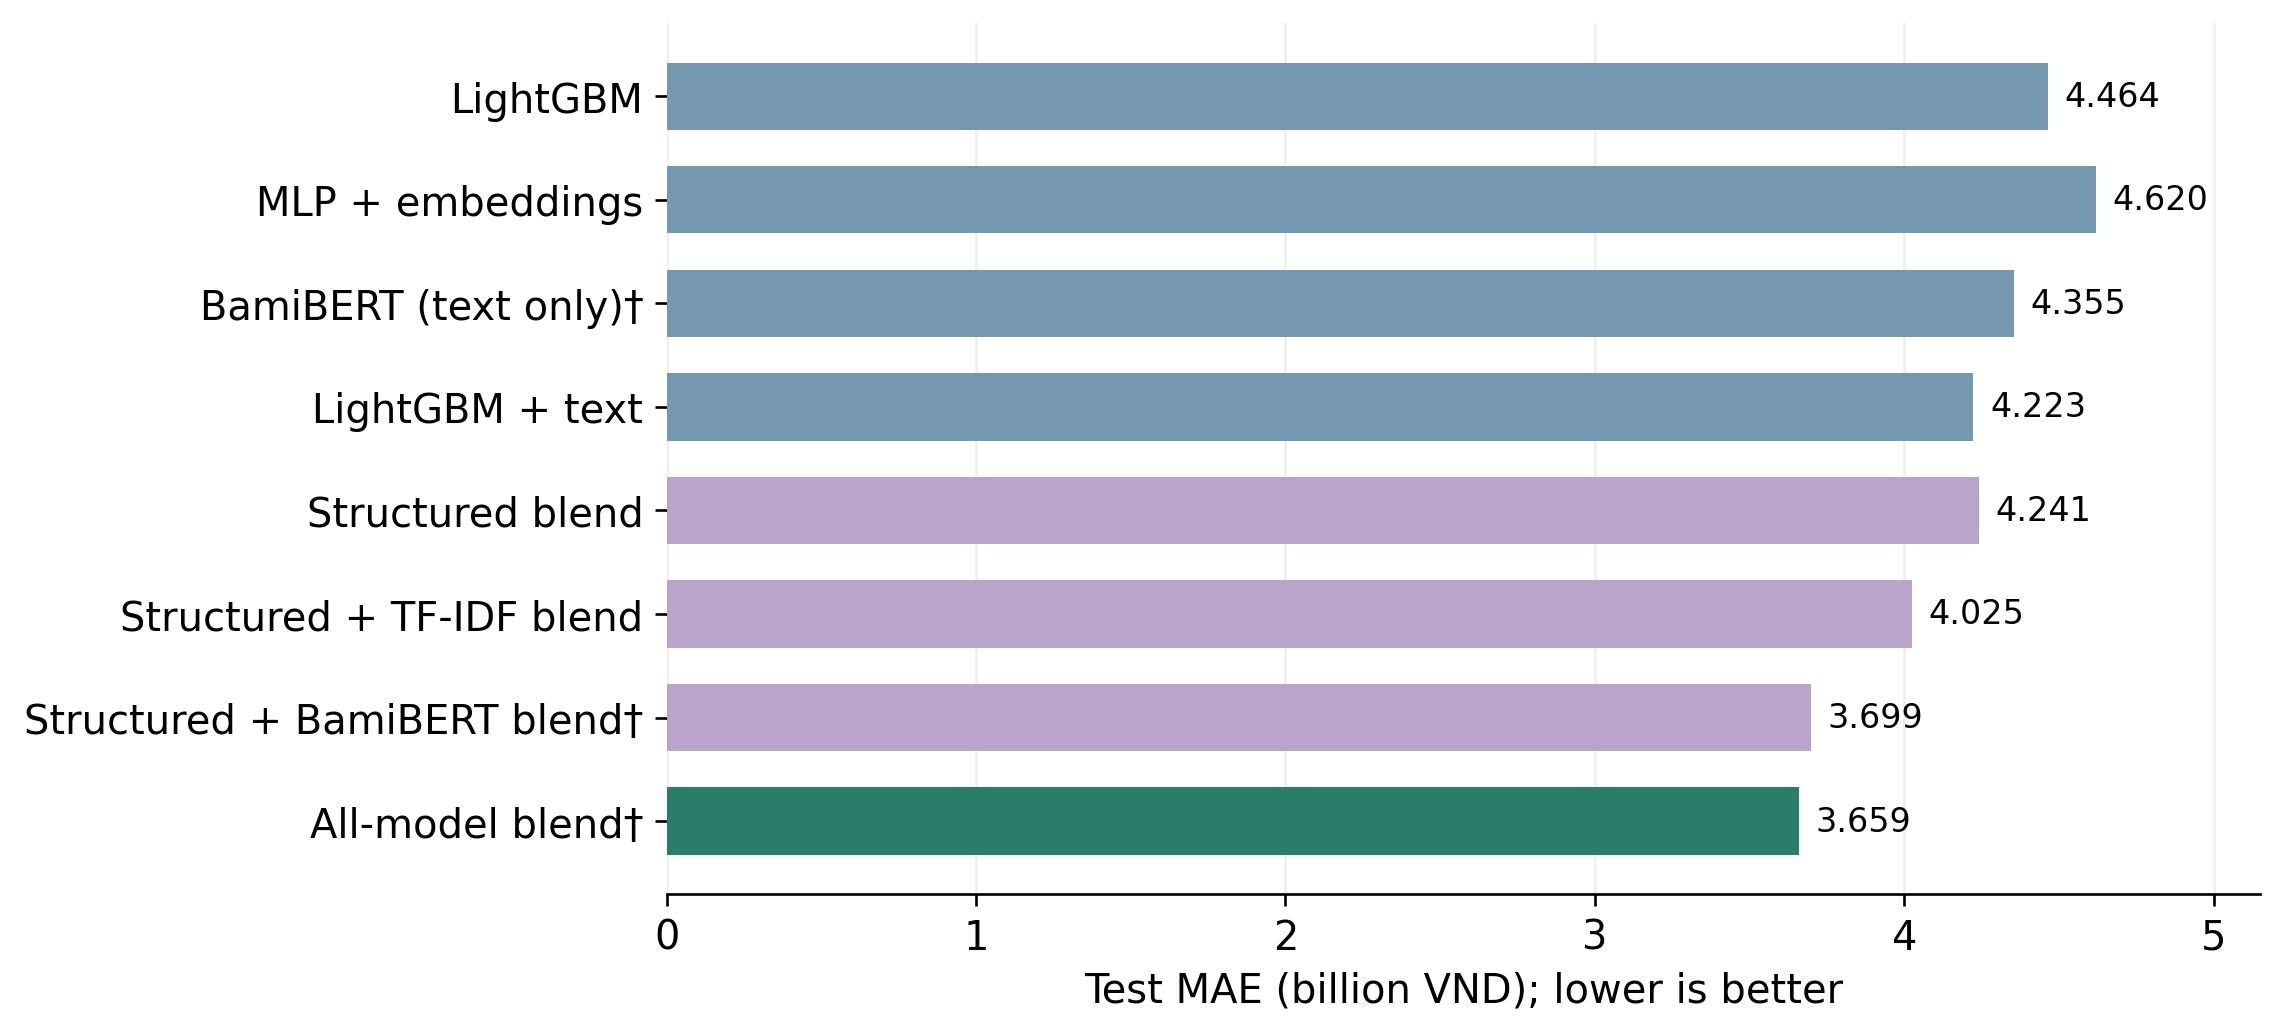
\includegraphics[width=0.82\textwidth]{figures/conclusion_model_comparison.png}
\caption[Individual models and blends: test MAE]{Held-out test MAE for selected predictors and blends; lower is better. $\dagger$ Results involving BamiBERT await checkpoint-reload verification.}
\label{fig:model-comparison}
\end{figure}

The all-model blend reduces MAE by 13.4\% relative to text-enhanced LightGBM and by 18.0\% relative to structured LightGBM. Its gain over the smaller structured--BamiBERT blend is only 1.1\%. Stacking combines complementary predictions~\cite{wolpert1992stacked}, but inference-time measurements are needed to assess the cost of this final increment in accuracy.

\subsection{Limitations}
\label{subsec:evaluation-limitations}

\paragraph{Data quality and population coverage.}
The target is an advertised asking price, without verified transactions or reliable sale/rental labels. Ho Chi Minh City and Hanoi account for approximately 71\% of the full analytical dataset. Inaccurate values may survive filtering, and revised titles or prices can leave repeated properties across partitions. Accuracy is not established separately for each province, property type, price range, or future period.

\paragraph{Model-selection and stacking protocol.}
Only one temporal holdout is evaluated, and final fitting populations differ. Validation is reused for tuning, stopping, and blend fitting. The text-derived feature uses ordinary five-fold prediction with a vocabulary fitted before the folds, rather than forward-chaining preprocessing. Repeated seeds, additional time windows, and uncertainty intervals are needed to assess stability and statistical significance.

\paragraph{Text leakage and checkpoint verification.}
Monetary-clause filtering can leave misspelled price expressions and numeric fragments, especially when other numbers are retained. BamiBERT checkpoint reload also reports missing and unexpected LayerNorm parameter names, distinct from a new regression head. The parameter mapping and residual price leakage require verification before stronger claims about BamiBERT or its blends. One training epoch does not establish the best performance attainable with longer fine-tuning.

\endgroup
